\documentclass{beamer}
\mode<presentation>

\usepackage{enumerate}

\title{Young Tableaux: una implementazione}
\author[Campagni]{Candidato: Alessandro Campagni \medskip \\Relatore:
  Marco Maggesi}
\date{}

\usetheme{CambridgeUS}

\begin{document}

\begin{frame}
\titlepage
\end{frame}

%% \frame{\tableofcontents}

\section{Preliminari}
\subsection{Diagrammi di Young}

\begin{frame}
\frametitle{Diagramma di Young}
\begin{columns}[T]
\column{5cm}
\includegraphics[width=0.6\textwidth]{images/YoungDiagram.pdf}
\column{5cm}
$11=4+3+2+1+1$
\end{columns}
\end{frame}

%% \begin{frame}
%% \frametitle{Diagramma coniugato}
%% \begin{columns}[T]
%% \column{5cm}
%% 
\includegraphics[height=0.6\textwidth]{images/YoungDiagramTransposed.pdf}
%% \column{5cm}
%% $11=5+3+2+1$
%% \end{columns}
%% \end{frame}

\begin{frame}
\frametitle{Skew diagram}
\centering
\begin{columns}
\begin{column}{3.3cm}
\includegraphics[width=0.7\textwidth]{images/skew_diag_1.pdf}\\
$\lambda=(5,3,2)$
\end{column}
\begin{column}{3.3cm}
\includegraphics[width=0.7\textwidth]{images/skew_diag_2.pdf}\\
$\mu=(2,1)$
\end{column}
\begin{column}{3.3cm}
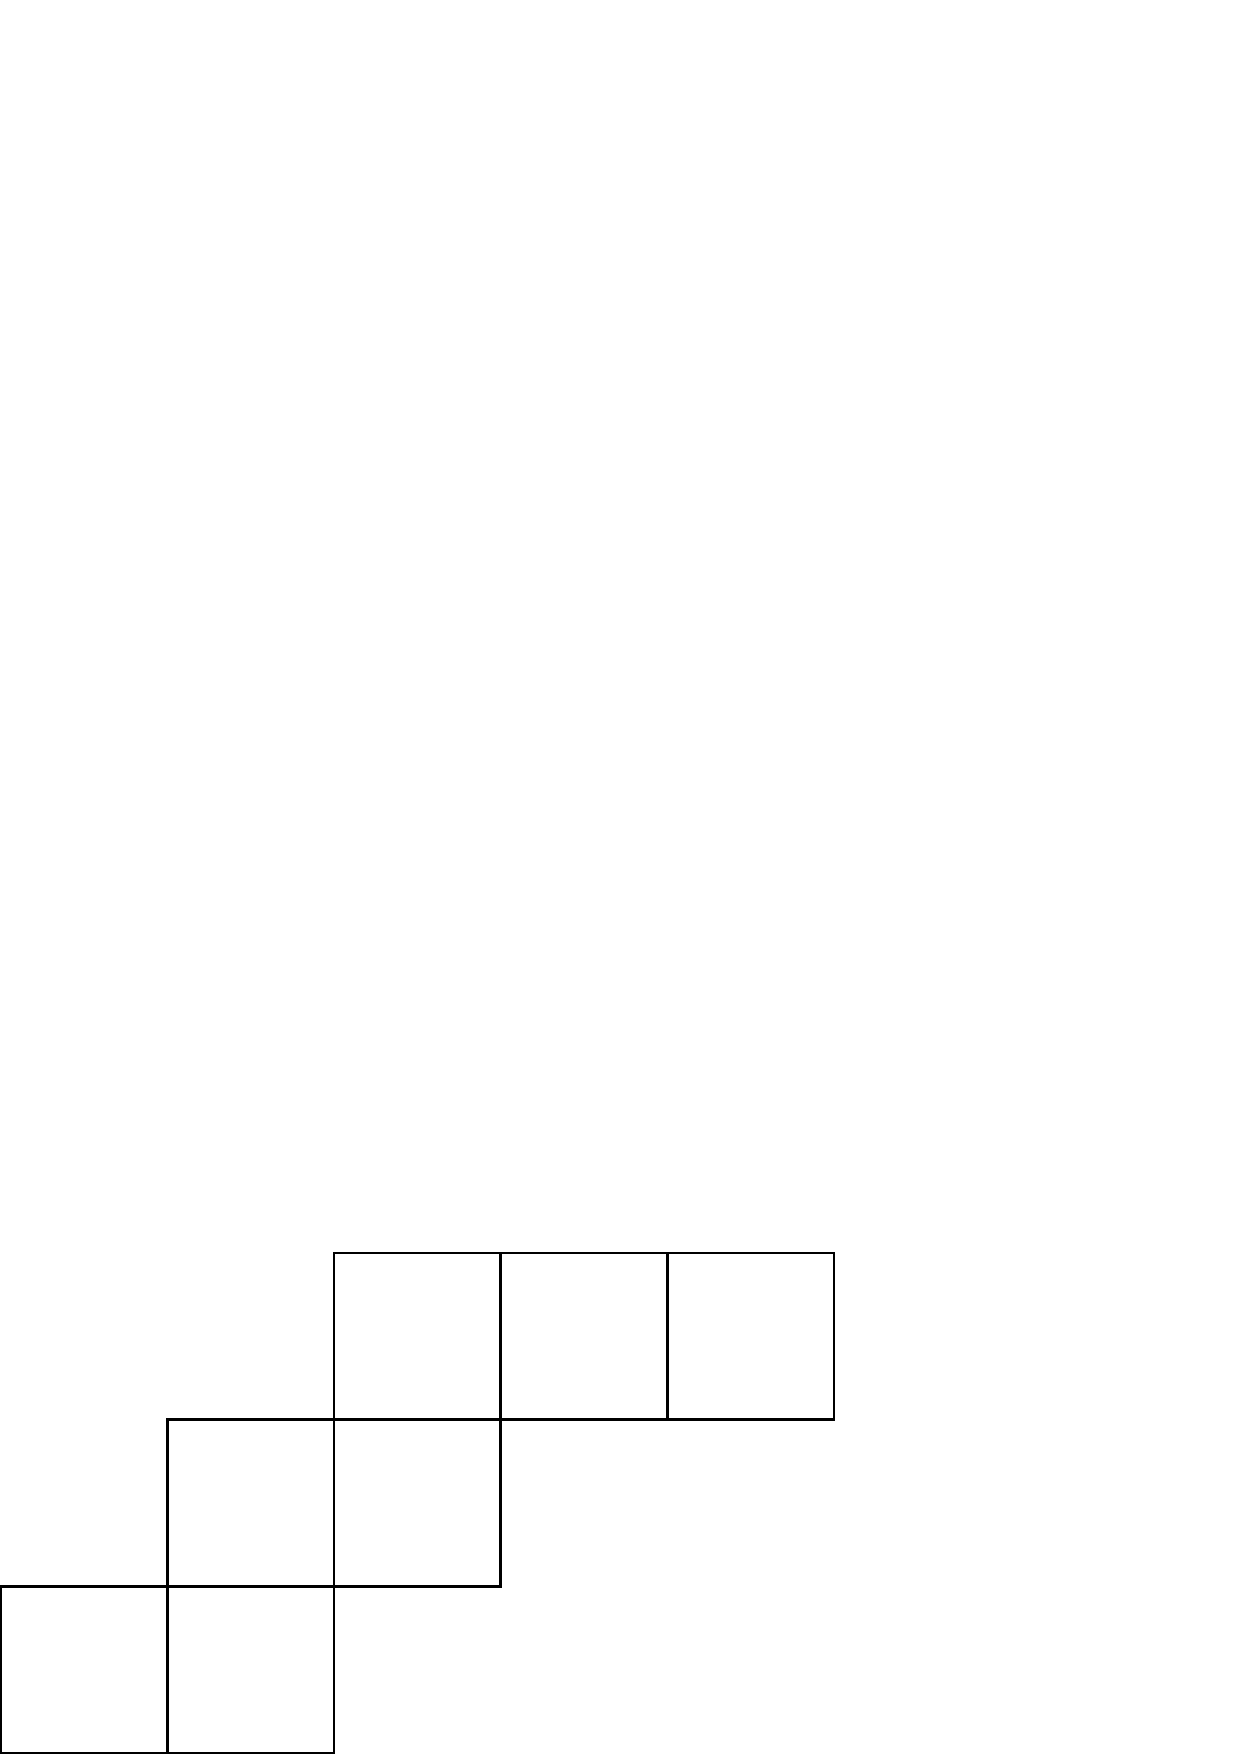
\includegraphics[width=0.7\textwidth]{images/skew_diag_3.pdf}\\
$\lambda / \mu$
\end{column}
\end{columns}
\end{frame}

\subsection{Young tableaux}

\begin{frame}
\frametitle{Young tableau}
\begin{columns}
\column{5cm}
\includegraphics[width=0.7\textwidth]{images/tableau.pdf}
\column{5cm}
\begin{enumerate}[(i)]
\item $T^i_j \leq T^i_{j+1}$
\item $T^i_j < T^{i+1}_j$
\end{enumerate}
\end{columns}
\end{frame}

\begin{frame}
\frametitle{Row bumping}
\centering
\begin{columns}[t]
\begin{column}{3.3cm}
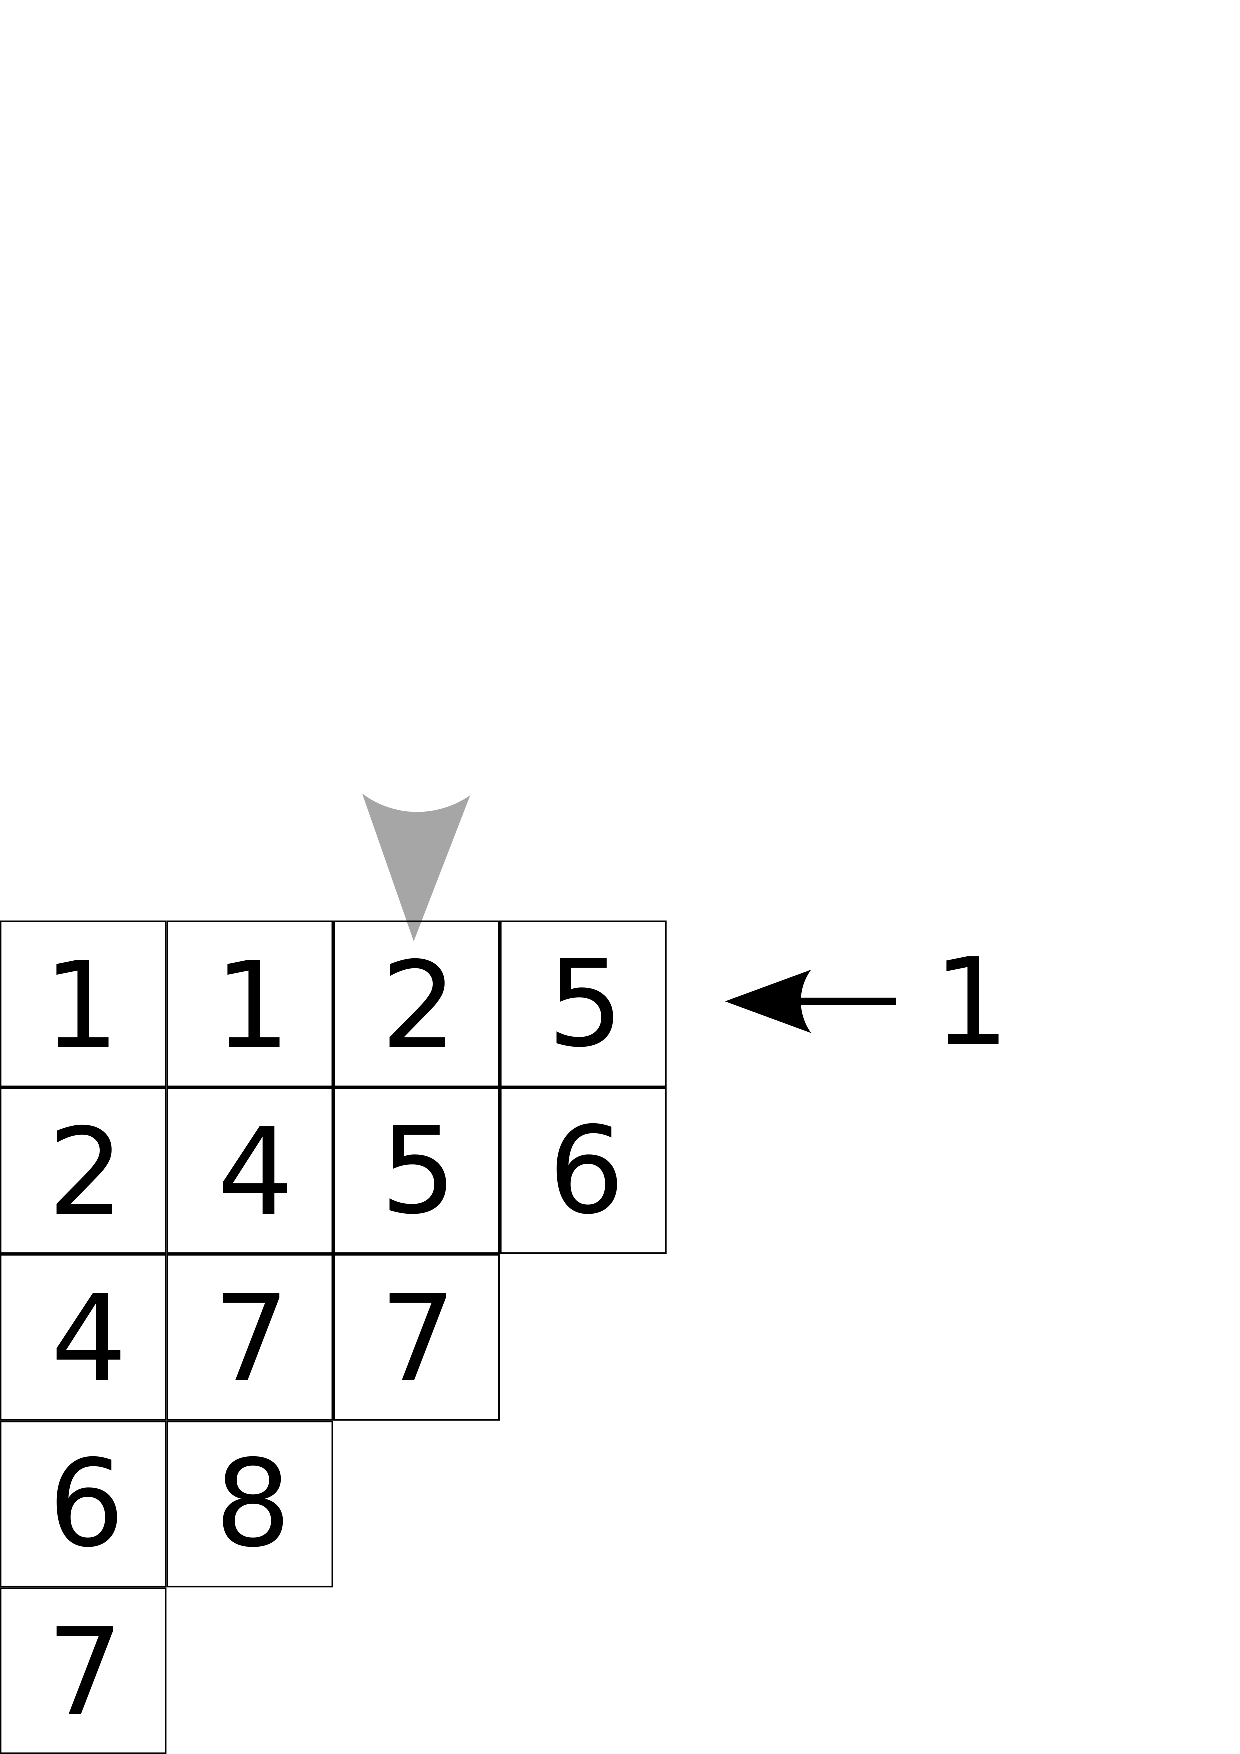
\includegraphics[height=0.7\textwidth]{images/bump_1.pdf}\\
\includegraphics[height=0.6\textwidth]{images/bump_4.pdf}
\end{column}
\begin{column}{3.3cm}
\includegraphics[height=0.6\textwidth]{images/bump_2.pdf}\\
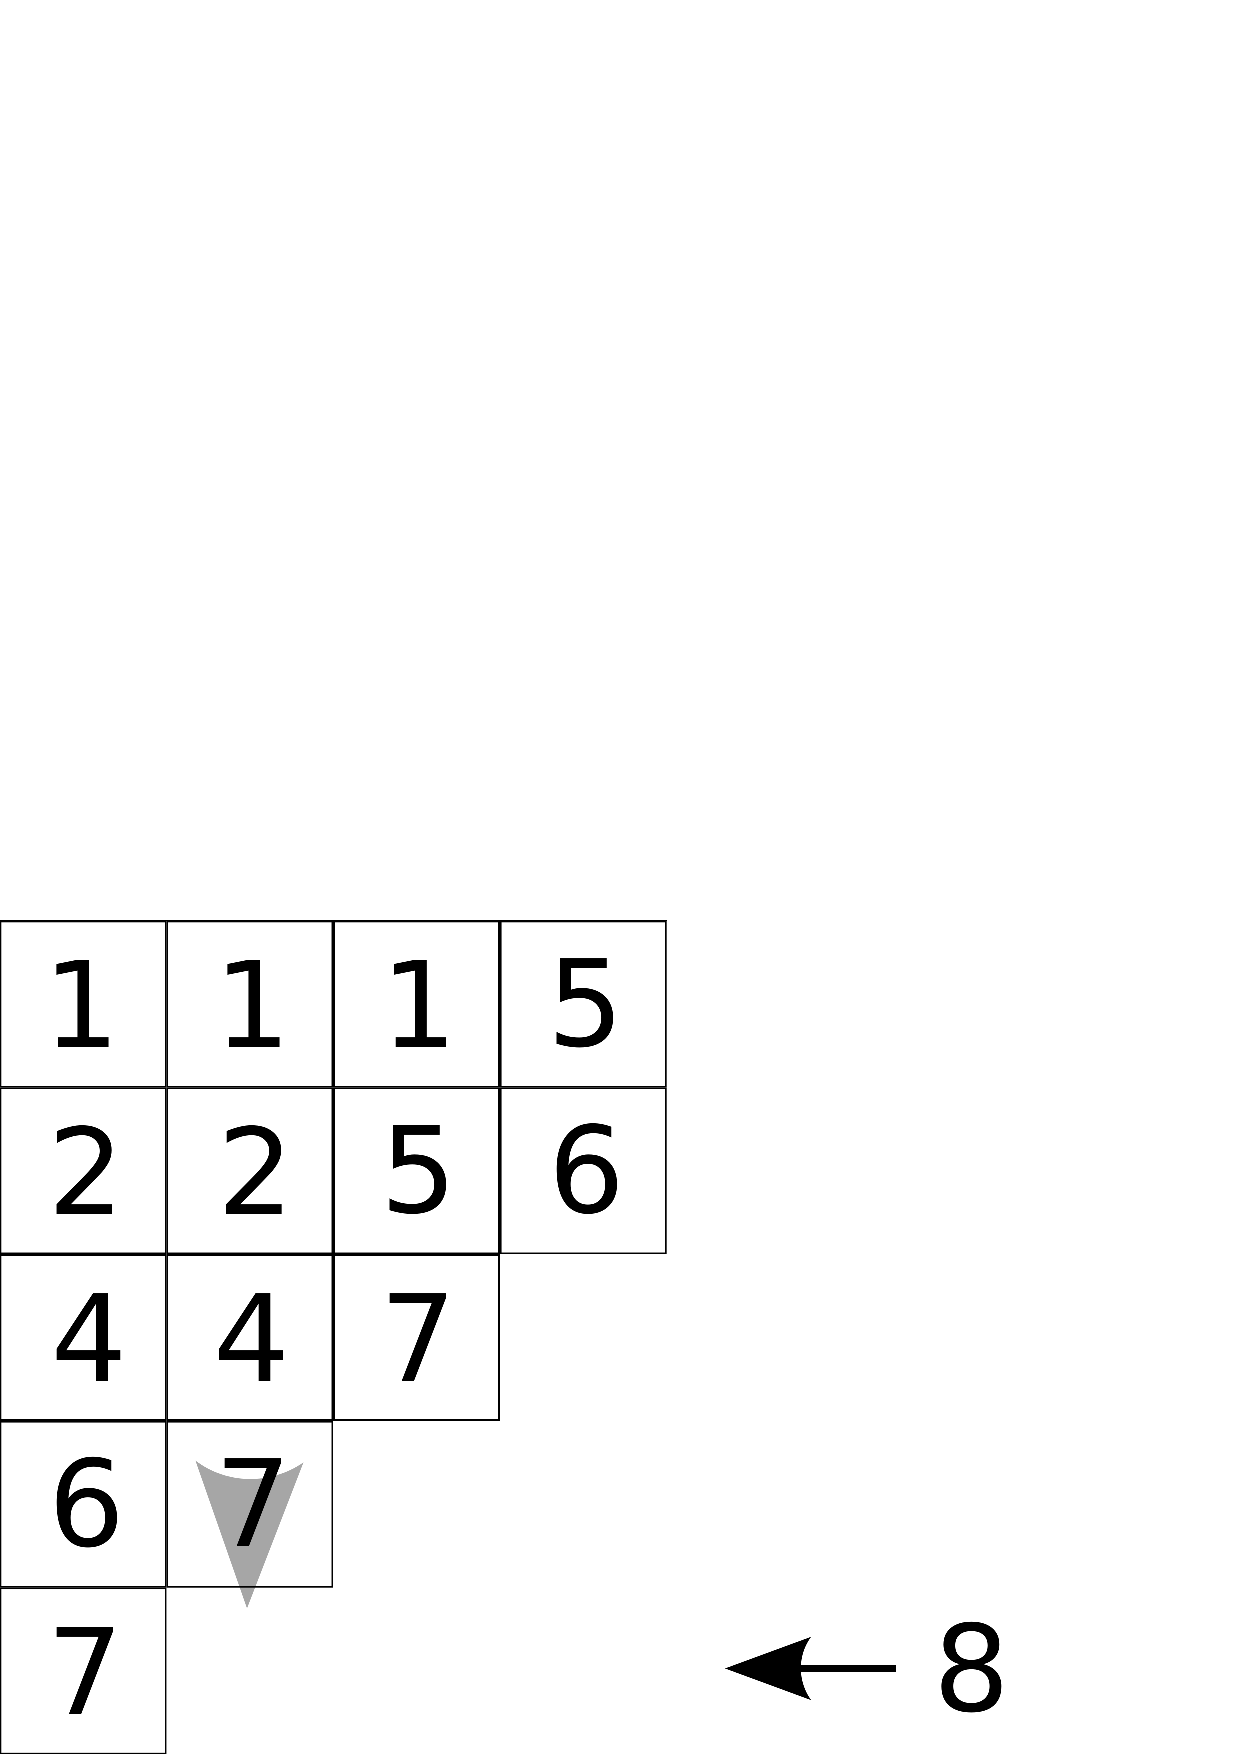
\includegraphics[height=0.6\textwidth]{images/bump_5.pdf}
\end{column}
\begin{column}{3.3cm}
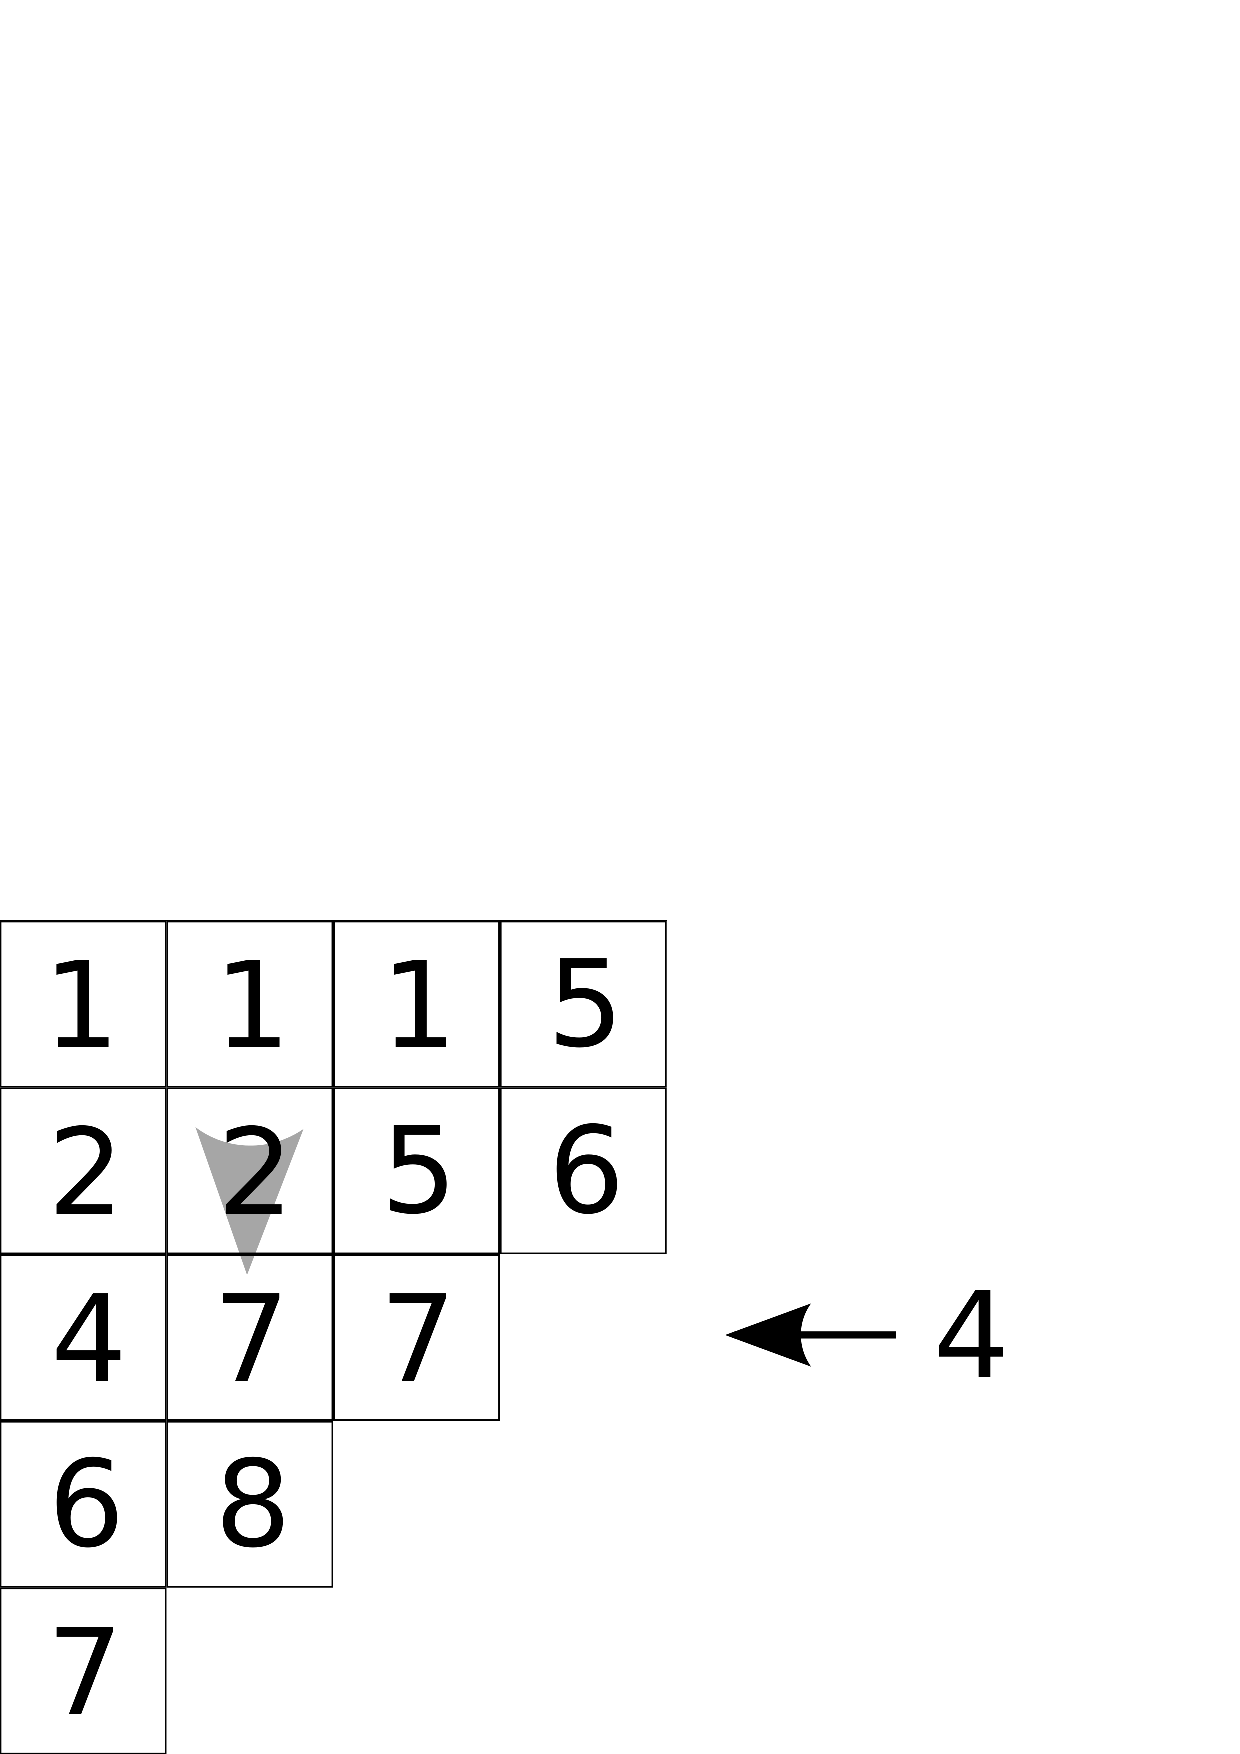
\includegraphics[height=0.6\textwidth]{images/bump_3.pdf}\\
\includegraphics[height=0.6\textwidth]{images/bump_6.pdf}
\end{column}
\end{columns}
\end{frame}

\begin{frame}
\frametitle{Prodotto di tableaux}
\centering
\begin{columns}[t]
\begin{column}{5cm}
\includegraphics[width=0.7\textwidth]{images/prod_1.pdf}\\
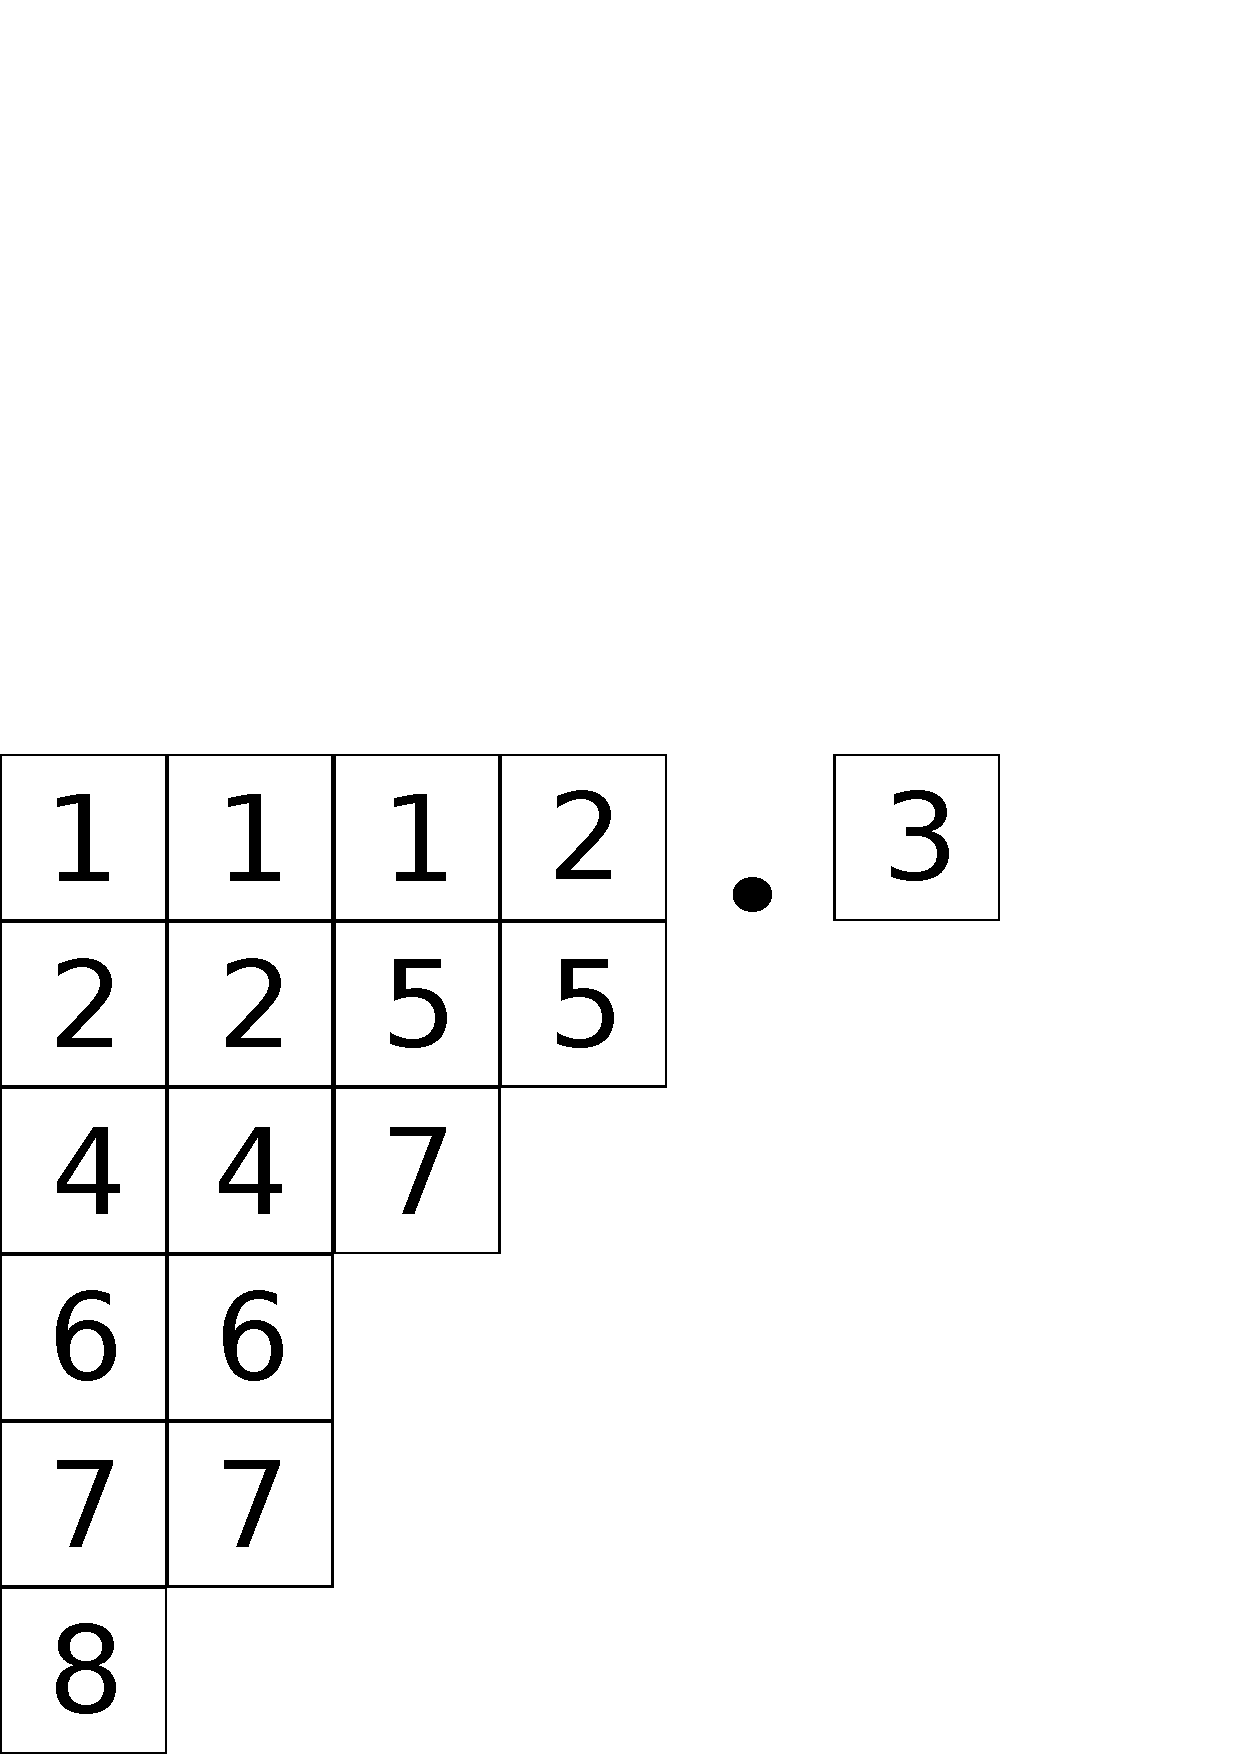
\includegraphics[width=0.6\textwidth]{images/prod_3.pdf}
\end{column}
\begin{column}{5cm}
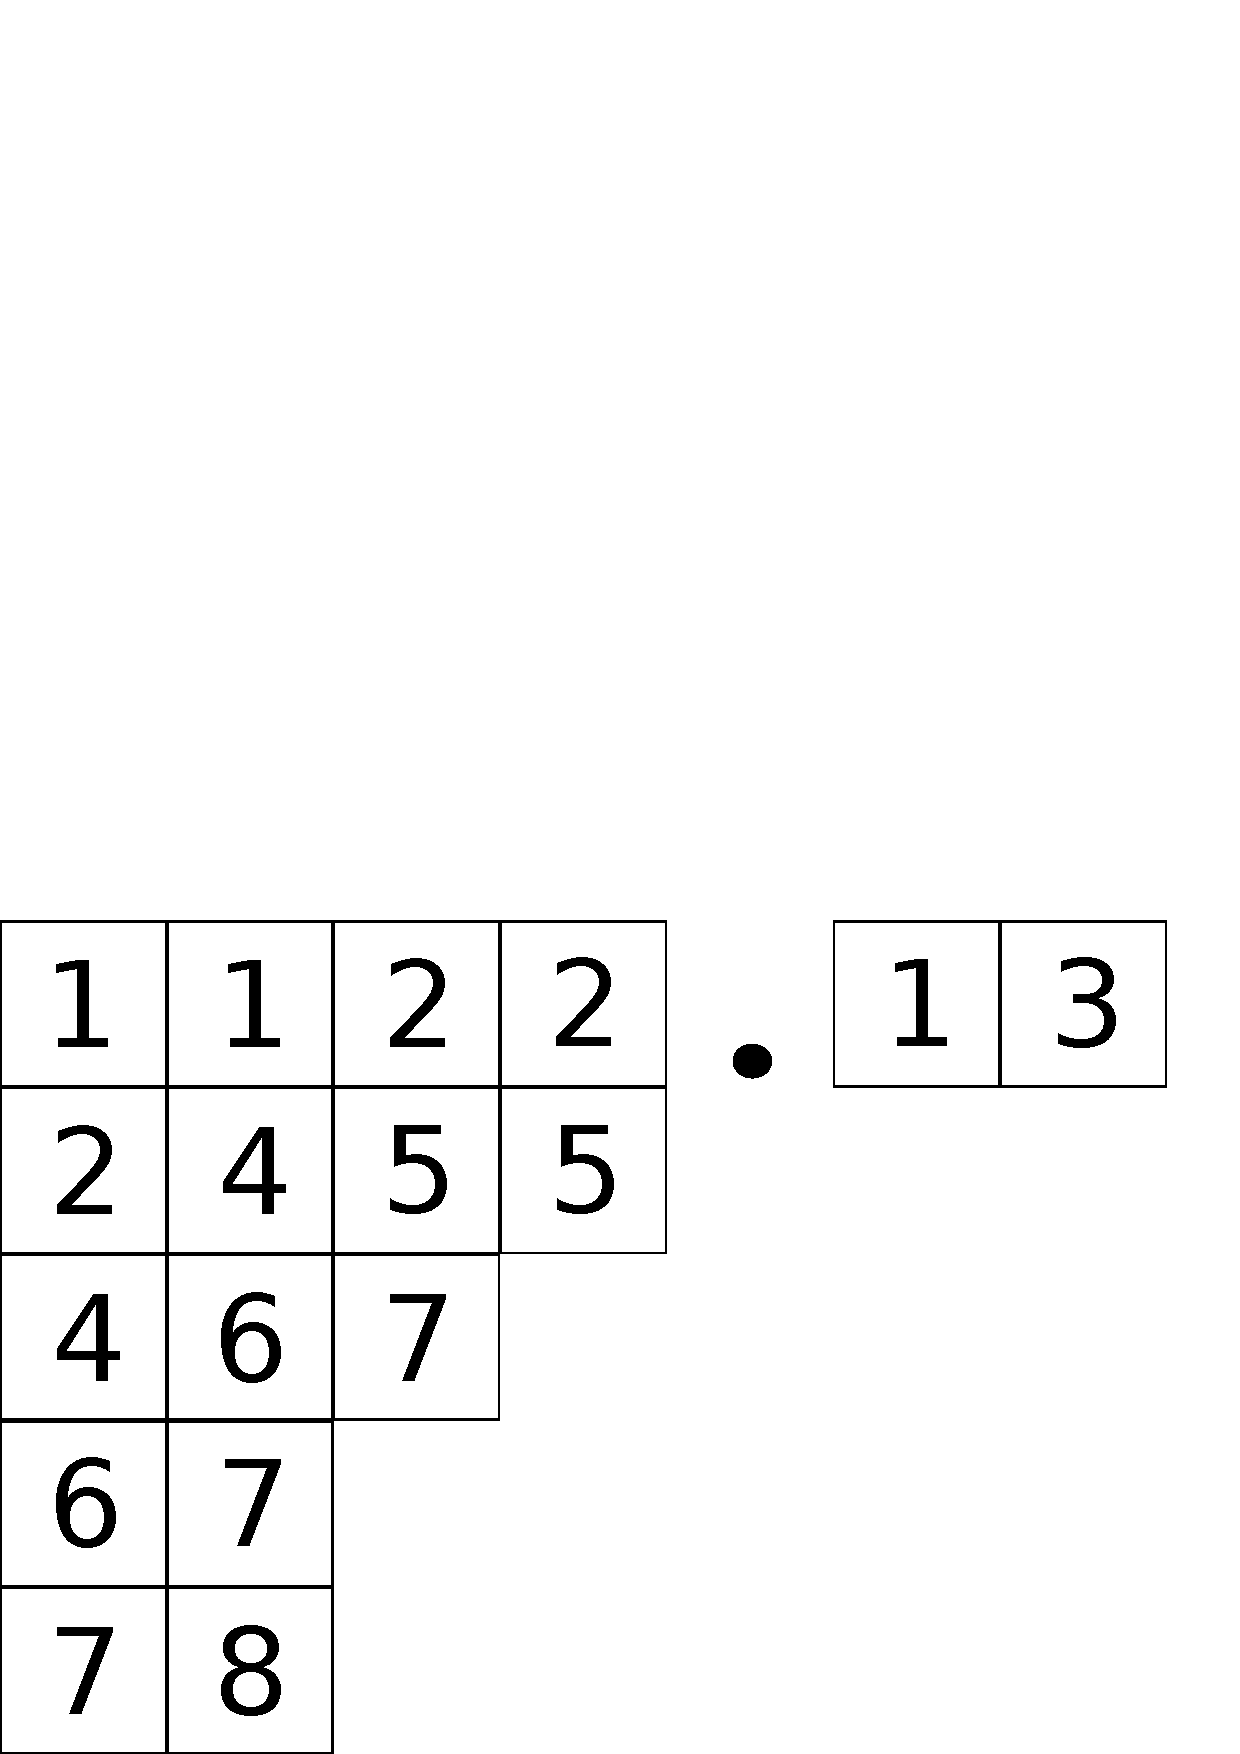
\includegraphics[width=0.7\textwidth]{images/prod_2.pdf}\\
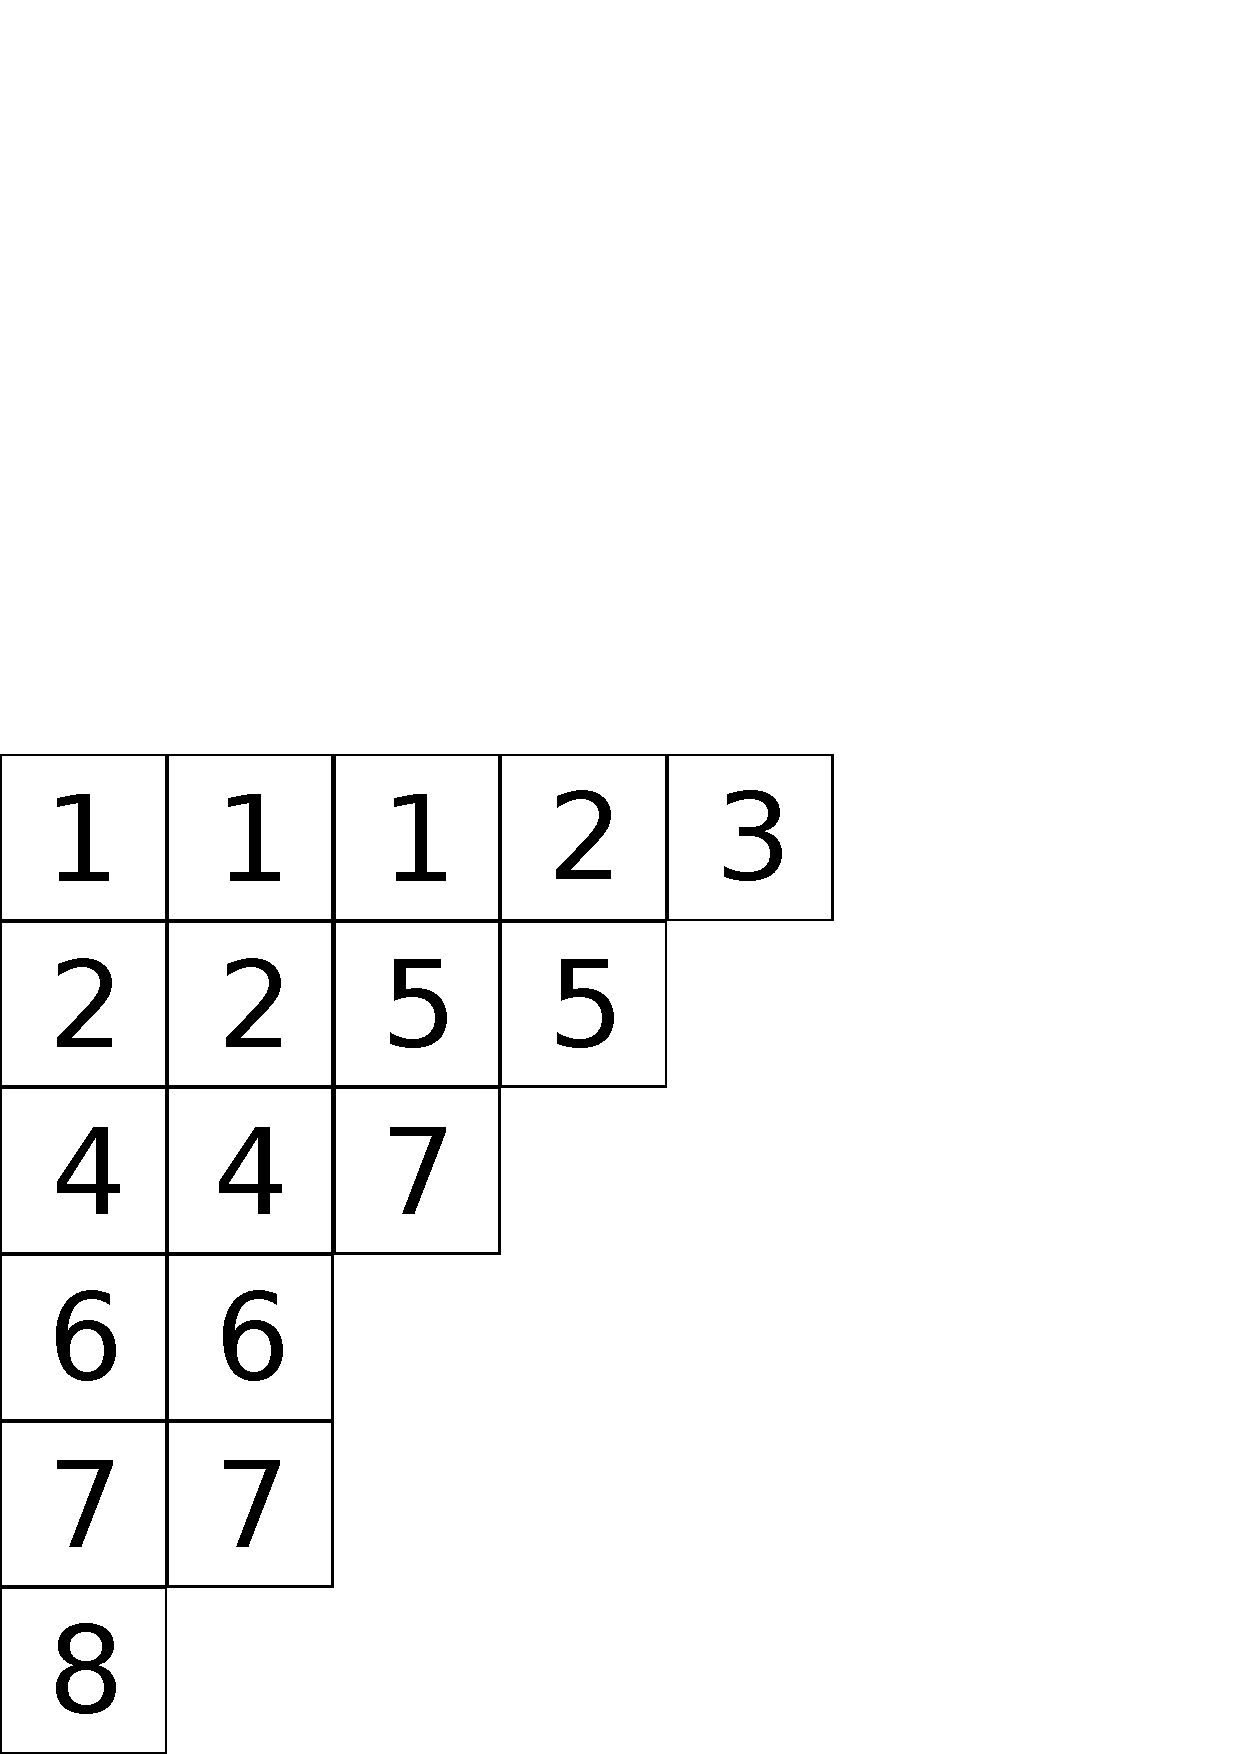
\includegraphics[width=0.5\textwidth]{images/prod_4.pdf}
\end{column}
\end{columns}
\end{frame}

%% \subsection{Skew tableau}

\section{Polinomi di Schur}

\subsection{Definizione}

\begin{frame}
\frametitle{Monomio di un tableau}
\centering
\begin{columns}
\begin{column}{5cm}
%% \begin{overprint}
%% \onslide<2->
\includegraphics[width=0.4\textwidth]{images/tableau.pdf}
%% \end{overprint}
%% \begin{overprint}
%% \onslide<3->
\Large $x_1^2 x_2^2 x_4^2 x_5^2 x_6^2 x_7^3 x_8$
%% \end{overprint}
\end{column}
\begin{column}{5cm}
$x^T = \prod\limits_{i = 1}^m x_i^{c(i)}$
\end{column}
\end{columns}
\end{frame}

\subsection{L'algoritmo}

\begin{frame}
\frametitle{Polinomio di Schur}
\begin{columns}[T]
\begin{column}{5cm}
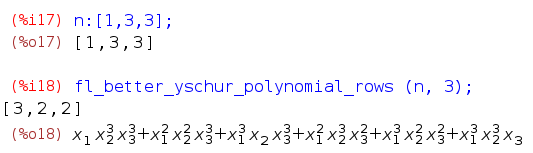
\includegraphics[width=\textwidth]{images/schur_poly_demo.png}
\end{column}
\begin{column}{5cm}

\begin{columns}[T]
\begin{column}{2.5cm}
\begin{overprint}[\textwidth]
\onslide<2->
\includegraphics[height=0.4\textwidth]{images/yschur_1.pdf}
\end{overprint}
\end{column}
\begin{column}{2.5cm}
\begin{overprint}[\textwidth]
\onslide<3->

\includegraphics[height=0.4\textwidth]{images/yschur_2.pdf}
\end{overprint}
\end{column}
\end{columns}

\begin{overprint}[\textwidth]
\begin{columns}[b]
\column{1.66cm}
\includegraphics<4->[height=0.6\textwidth]{images/yschur_3.pdf}
\column{1.66cm}
\includegraphics<4>[height=0.6\textwidth]{images/yschur_4.pdf}
\includegraphics<5->[height=0.6\textwidth]{images/yschur_6.pdf}
\column{1.66cm}
\includegraphics<4>[height=0.6\textwidth]{images/yschur_5.pdf}
\includegraphics<5->[height=0.6\textwidth]{images/yschur_7.pdf}
\end{columns}
\end{overprint}

\begin{overprint}[\textwidth]
\onslide<6->
\begin{columns}[c]
\column{1.66cm}
\includegraphics[height=0.6\textwidth]{images/yschur_8.pdf}
\column{1.66cm}
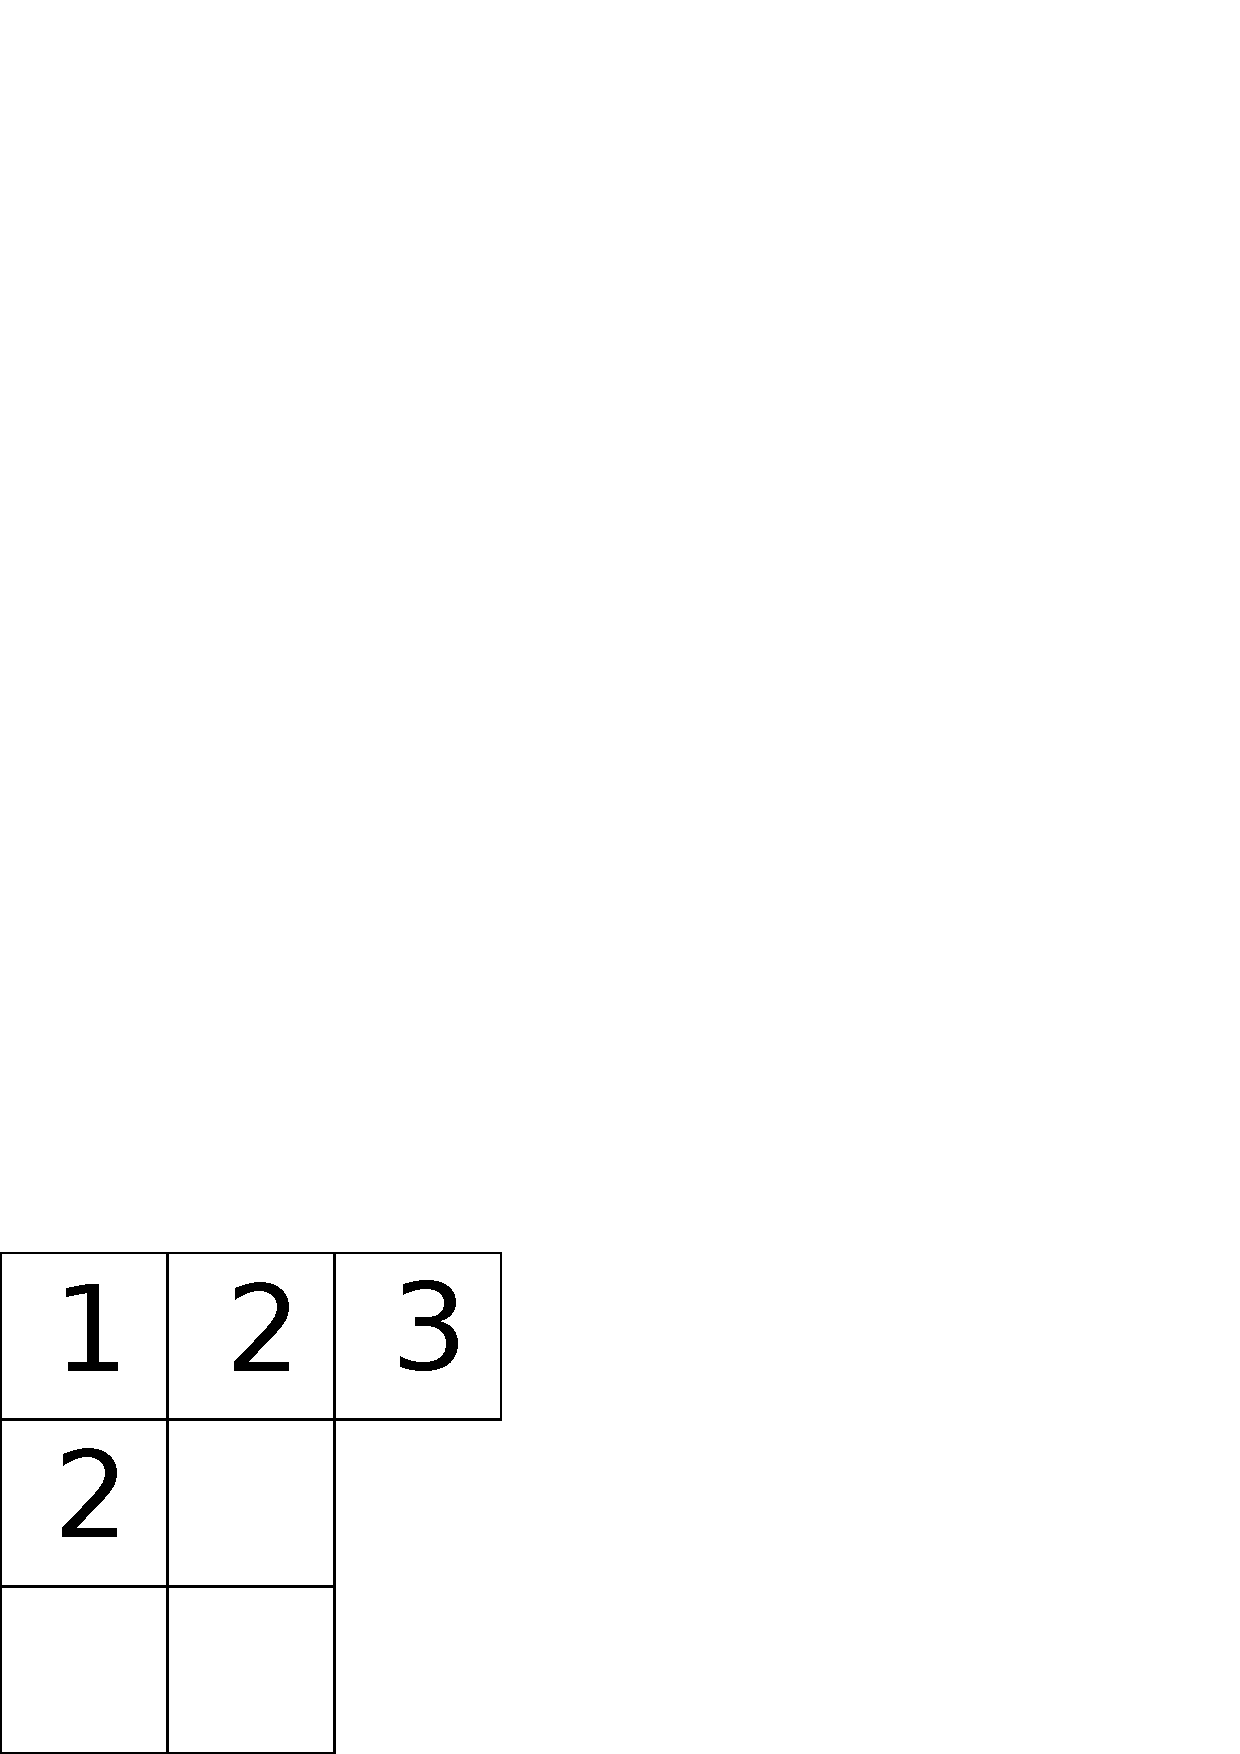
\includegraphics[height=0.6\textwidth]{images/yschur_9.pdf}
\column{1.66cm}
\includegraphics[height=0.6\textwidth]{images/yschur_10.pdf}
\end{columns}
\end{overprint}

\end{column}
\end{columns}
\end{frame}

\begin{frame}
\frametitle{Polinomio di Schur}
\begin{columns}[c]
\column{3.33cm}
%% \includegraphics<1>[height=0.7\textwidth]{images/yschur_11.pdf}\\
%% \includegraphics<1>[height=0.7\textwidth]{images/yschur_12.pdf}
\includegraphics<1->[height=0.5\textwidth]{images/yschur_11.pdf}\\
\includegraphics<1->[height=0.5\textwidth]{images/yschur_12.pdf}
\column{3.33cm}
%% \includegraphics<1>[height=0.7\textwidth]{images/yschur_13.pdf}\\
%% \includegraphics<1>[height=0.7\textwidth]{images/yschur_14.pdf}
\includegraphics<1->[height=0.5\textwidth]{images/yschur_13.pdf}\\
\includegraphics<1->[height=0.5\textwidth]{images/yschur_14.pdf}
\column{3.33cm}
%% \includegraphics<1>[height=0.7\textwidth]{images/yschur_15.pdf}\\
%% \includegraphics<1>[height=0.7\textwidth]{images/yschur_16.pdf}
\includegraphics<1->[height=0.5\textwidth]{images/yschur_15.pdf}\\
\includegraphics<1->[height=0.5\textwidth]{images/yschur_16.pdf}
\end{columns}
\onslide<1->{\Large$$x_{1}\,x_{2}^3\,x_{3}^3+x_{1}^2\,x_{2}^2\,x_{3}^3+x_{1}^3\,x_{2}\,x_{3}^3+x_{1}^2\,x_{2}^3\,x_{3}^2+x_{1}^3\,x_{2}^2\,x_{3}^2+x_{1}^3\,x_{2}^3\,x_{3}$$}
\end{frame}

\section{Littlewood-Richardson}

\subsection{I numeri di Littlewood-Richardson}

\begin{frame}
\frametitle{``Contare'' i prodotti di tabelle}
\begin{enumerate}[(i)]
\item $\lambda \vdash n$, $\mu \vdash m$, $\nu \vdash r$
\item $V$ tableau su $\nu$ 
\item $c_{\lambda \mu}^\nu=|\{ (T,U) \mid V = T \cdot U; U,T \text{
  tableaux su } \lambda \text{ e } \mu \text{ risp.}\}|=?$
\item $c_{\lambda, \mu}^\nu$ non dipende da $V$ ma solo da
  $\nu, \lambda, \mu$
\item $S_{\lambda}[m] \cdot S_{\mu}[m] =\sum\limits_{\nu}
  c_{\lambda \mu}^{\nu} S_{\nu}[m]$\\
$\implies s_{\lambda}(x_1,\ldots,x_m) \cdot s_{\mu}(x_1,\ldots,x_m) =
\sum\limits_{\nu} c_{\lambda \mu}^{\nu} s_{\nu}(x_1,\ldots,x_m)$
\end{enumerate}
\end{frame}

\begin{frame}
\frametitle{Skew tableaux di Littlewood-Richardson}
\begin{columns}[T]
\column{5cm}
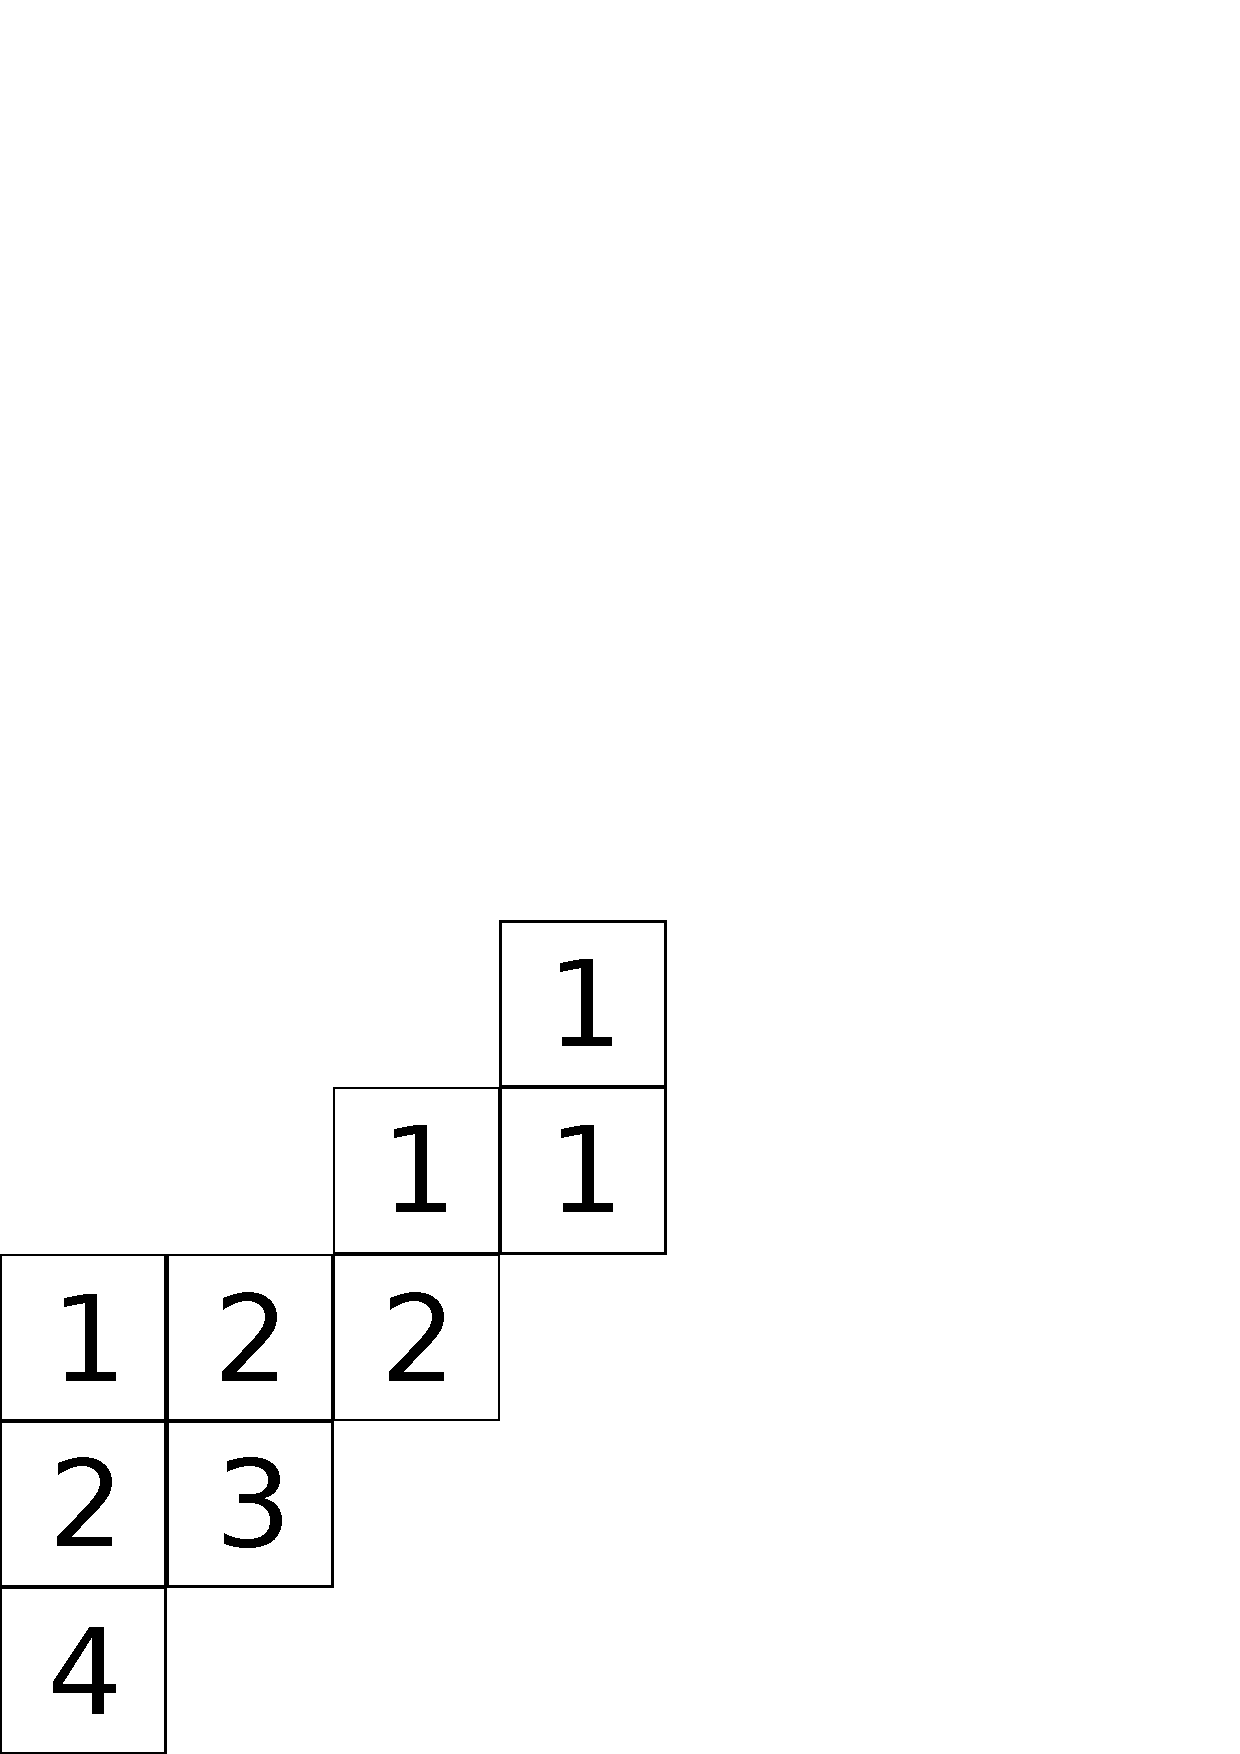
\includegraphics[width=0.8\textwidth]{images/littlewood-richardson_skew_tableau.pdf}
\column{5cm}
\begin{enumerate}[(i)]
\item skew tableau $T$
\item $w(T)$ reverse lattice order
\item \emph{contenuto} $\mu=(3,3,1,1)$
\end{enumerate}
\end{columns}
\end{frame}

\begin{frame}
\frametitle{L'algoritmo}
\begin{block}{Proposizione}
Il numero di skew tableaux di Littlewood-Richardson che riempiono lo
skew diagram $\nu/\lambda$ con contenuto $\mu$ \`e $c_{\lambda \mu}^{\nu}$.
\end{block}
\begin{enumerate}[(i)]
\item determinare $\nu$ forma del prodotto dei possibili tableaux su
  $\lambda$ e $\mu$
\item skew tableaux di Littlewood-Richardson su $\nu / \lambda$ con
  contenuto $\mu$
\end{enumerate}
\end{frame}

\end{document}
